\appendix
\section{附录：附加题技术实现报告}

\subsection{任务说明与模型选择依据}

附加题要求结合 AI 技术，实现定位误差预测与补偿，并说明模型选择、数据处理、训练细节、补偿步骤、效果验证和改进方向。本项目选择线性回归中的岭回归模型作为误差补偿模型，主要原因如下：

\begin{itemize}
\item 模型结构简单，回归系数具有可解释性，便于分析卫星数、DOP、残差等特征与定位误差之间的关系。
\item 训练样本来自本实验生成的连续定位结果，特征维度较低，线性模型可作为稳定的基准方法。
\item 岭回归在普通最小二乘基础上加入微小正则项，可以减弱特征相关性导致的矩阵病态问题。
\item 为保持项目依赖精简，代码采用项目内手写矩阵方程求解，形式上等价于常见机器学习库中的 Ridge 回归。
\end{itemize}

\subsection{数据处理过程}

模型训练数据来自 6 组连续定位结果，共 17280 条样本，满足“至少 3 组不同场景 RINEX 数据解算结果”的要求。训练脚本读取各数据集的 \texttt{results.csv}，将所有历元结果汇总后，按 70\%/30\% 划分训练集和测试集。

\begin{table}[H]
\centering
\small
\begin{tabular}{lcc}
\toprule
数据来源 & 系统类型 & 样本数 \\
\midrule
BJFS & GPS & 2880 \\
DAEJ & GPS & 2880 \\
HKSL & GPS & 2880 \\
TWTF & GPS & 2880 \\
TWTF & BDS & 2880 \\
TWTF & GPS+BDS & 2880 \\
\bottomrule
\end{tabular}
\caption{附加题训练数据来源}
\end{table}

输入特征选取连续定位结果中与误差相关的解算状态量，包括：

\begin{table}[H]
\centering
\small
\begin{tabular}{p{0.28\linewidth}p{0.62\linewidth}}
\toprule
特征 & 含义 \\
\midrule
\texttt{used\_sats} & 当前历元参与解算的卫星数量，反映观测冗余度。 \\
\texttt{pdop}, \texttt{gdop} & 几何精度因子，反映卫星空间构型对定位误差放大的影响。 \\
\texttt{residual\_rms\_m} & 后验残差 RMS，反映观测噪声和模型误差水平。 \\
\texttt{residual\_max\_m} & 最大后验残差，用于刻画可能存在的粗差或多路径影响。 \\
\texttt{clock\_bias\_m} & 接收机钟差估计值，可间接反映解算状态。 \\
\texttt{h} & 解算高程，高程方向误差对三维定位误差影响明显。 \\
\bottomrule
\end{tabular}
\caption{误差补偿模型输入特征}
\end{table}

预测标签为 ENU 三个方向误差：\texttt{east}、\texttt{north}、\texttt{up}。训练前对输入特征进行均值和标准差归一化，避免不同量纲导致某些特征在法方程中占主导。

\subsection{模型训练细节}

模型实现文件为 \texttt{src/ml\_compensation.py}，训练入口为 \texttt{scripts/train\_error\_model.py}。训练流程如下：

\begin{enumerate}
\item 读取 6 组连续定位 CSV 文件，合并为统一样本表。
\item 使用确定性打乱方式划分训练集和测试集，训练集 12096 条，测试集 5184 条。
\item 计算训练集特征均值与标准差，并对训练集和测试集使用相同参数归一化。
\item 分别对 \texttt{east}、\texttt{north}、\texttt{up} 训练三组岭回归系数。
\item 保存模型参数到 \texttt{results/ml\_compensation/linear\_model.json}，保存指标到 \texttt{metrics.csv}，生成精度对比图。
\end{enumerate}

模型形式为：

\begin{verbatim}
y = beta0 + beta1*x1 + beta2*x2 + ... + betaN*xN
\end{verbatim}

岭回归法方程为：

\begin{verbatim}
(X^T X + lambda I) beta = X^T y
\end{verbatim}

其中偏置项不参与正则化，\texttt{lambda} 取较小值用于增强数值稳定性。线性方程求解使用手写高斯消元，与主项目中“核心算法手写实现”的要求保持一致。

\subsection{补偿实现步骤}

误差补偿流程与原有连续定位结果衔接，具体步骤为：

\begin{enumerate}
\item 原始定位 pipeline 先输出每个历元的坐标、DOP、卫星数、残差和 ENU 误差。
\item 误差模型读取单历元特征并执行 \texttt{model.predict(row)}，得到预测误差 \texttt{pred\_east}、\texttt{pred\_north}、\texttt{pred\_up}。
\item 对原始 ENU 误差进行补偿：
\begin{verbatim}
comp_east  = east  - pred_east
comp_north = north - pred_north
comp_up    = up    - pred_up
\end{verbatim}
\item 根据补偿后的 ENU 误差重新计算水平误差与三维误差。
\item 输出补偿前后 RMS、均值、最大误差，并绘制精度对比图。
\end{enumerate}

当前项目以脚本方式集成该流程：连续定位输出 \texttt{results.csv} 后，训练脚本可自动完成特征读取、模型训练、预测补偿和指标输出。模型参数保存为 JSON，后续可进一步加载到 GUI 或实时 pipeline 中，实现运行过程中的在线误差提示与补偿显示。

\subsection{效果验证与分析}

测试集用于验证补偿效果，评价指标包括水平误差和三维误差的 RMS、均值、最大值。结果如下：

\begin{table}[H]
\centering
\scriptsize
\begin{tabular}{p{0.11\linewidth}p{0.20\linewidth}p{0.21\linewidth}p{0.21\linewidth}p{0.11\linewidth}}
\toprule
数据划分 & 指标 & 原始误差 & 补偿后误差 & 改善率 \\
\midrule
训练集 & 水平 RMS/均值/最大值 & 4.472 / 3.118 / 53.206 & 2.613 / 2.091 / 20.837 & 41.57\% \\
训练集 & 三维 RMS/均值/最大值 & 5.736 / 4.709 / 59.987 & 3.416 / 2.875 / 26.348 & 40.44\% \\
测试集 & 水平 RMS/均值/最大值 & 4.464 / 3.121 / 46.940 & 2.585 / 2.074 / 12.463 & 42.08\% \\
测试集 & 三维 RMS/均值/最大值 & 5.716 / 4.703 / 52.348 & 3.373 / 2.856 / 16.552 & 40.99\% \\
\bottomrule
\end{tabular}
\caption{误差补偿前后精度指标对比，单位为 m}
\end{table}

\begin{figure}[H]
\centering
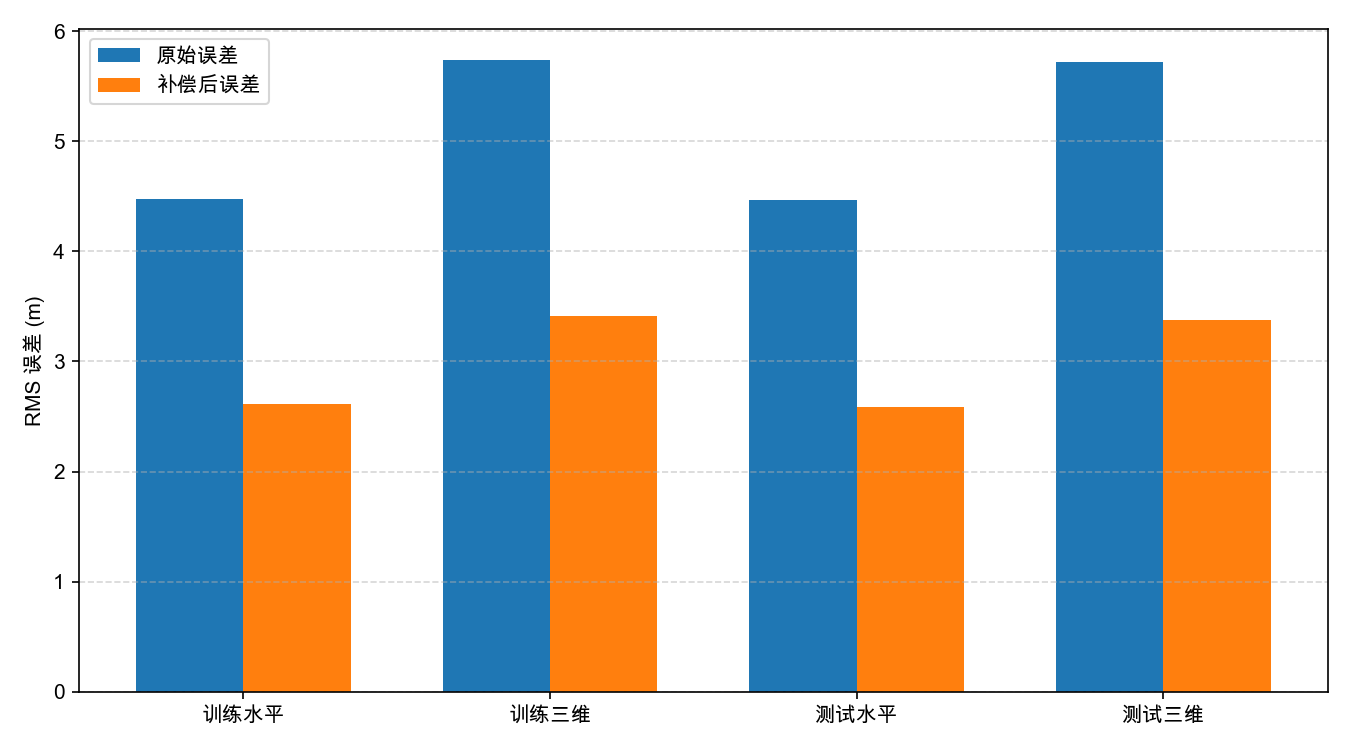
\includegraphics[width=0.60\linewidth]{figures/ml_compensation/compensation_comparison.png}
\caption{误差补偿前后 RMS 对比}
\end{figure}

从结果看，测试集三维 RMS 从 5.716 m 降至 3.373 m，改善率约为 40.99\%；测试集水平 RMS 从 4.464 m 降至 2.585 m，改善率约为 42.08\%。最大误差也明显下降，说明模型能够学习到一部分与 DOP、卫星数、残差和高程相关的系统性误差。

\subsection{优势、不足与改进方向}

线性回归误差补偿的优势是实现简单、运行速度快、参数可解释，适合作为传统 GNSS 解算后的轻量级增强模块。它可以利用定位解算过程中自然产生的 DOP、卫星数量和残差等指标，不需要额外传感器或复杂环境建模。

不足之处在于，线性模型只能表达近似线性关系，对遮挡、多路径、低高度角卫星和不同站点环境差异的非线性影响建模能力有限。此外，当前特征主要来自定位结果 CSV，尚未直接使用每颗卫星的 SNR/CN0、平均高度角、方位角分布等更细粒度信息。

后续改进方向包括：

\begin{itemize}
\item 加入 SNR/CN0、平均高度角、低高度角卫星比例、最大残差卫星等更丰富特征。
\item 使用随机森林或梯度提升树等非线性模型，与线性模型进行对比。
\item 采用跨站点留一验证，检验模型在未知站点上的泛化能力。
\item 将模型加载到 GUI 和连续定位 pipeline 中，实时显示补偿前后定位结果。
\end{itemize}

总体来看，附加题体现了 AI 技术与北斗定位软件开发的融合思路：传统算法负责完成物理模型明确的卫星位置、钟差、延迟修正和最小二乘定位；机器学习模型则利用历史解算结果学习残余误差规律，作为后处理模块进一步提升定位精度。
